\chapter{Experiments}
This chapter deals with the experiments, their design, execution and results.
\section{Experimental Design}
This section deals the specification of the Android benchmark app, used hardware, used framework, used model and how the measurements are conducted. 
\begin{figure}[H]
\centering


\tikzset{every picture/.style={line width=0.75pt}} %set default line width to 0.75pt        

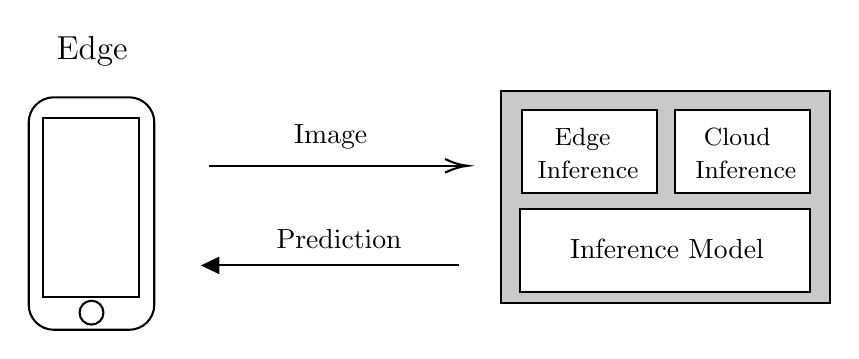
\begin{tikzpicture}[x=0.75pt,y=0.75pt,yscale=-1,xscale=1]
%uncomment if require: \path (0,175); %set diagram left start at 0, and has height of 175

%Shape: Rectangle [id:dp13292222689234756] 
\draw   (69.5,66) -- (115.5,66) -- (115.5,152) -- (69.5,152) -- cycle ;
%Rounded Rect [id:dp7897713915001106] 
\draw   (62.5,68.1) .. controls (62.5,61.42) and (67.92,56) .. (74.6,56) -- (110.9,56) .. controls (117.58,56) and (123,61.42) .. (123,68.1) -- (123,155.9) .. controls (123,162.58) and (117.58,168) .. (110.9,168) -- (74.6,168) .. controls (67.92,168) and (62.5,162.58) .. (62.5,155.9) -- cycle ;
%Shape: Circle [id:dp9670901006981827] 
\draw   (87,159.75) .. controls (87,156.57) and (89.57,154) .. (92.75,154) .. controls (95.93,154) and (98.5,156.57) .. (98.5,159.75) .. controls (98.5,162.93) and (95.93,165.5) .. (92.75,165.5) .. controls (89.57,165.5) and (87,162.93) .. (87,159.75) -- cycle ;
%Straight Lines [id:da9993479608904674] 
\draw    (149.48,89) -- (272,89) ;
\draw [shift={(274,89)}, rotate = 540] [color={rgb, 255:red, 0; green, 0; blue, 0 }  ][line width=0.75]    (10.93,-3.29) .. controls (6.95,-1.4) and (3.31,-0.3) .. (0,0) .. controls (3.31,0.3) and (6.95,1.4) .. (10.93,3.29)   ;

%Straight Lines [id:da5401559459790608] 
\draw    (147.48,137) -- (270,137) ;

\draw [shift={(145.48,137)}, rotate = 360] [fill={rgb, 255:red, 0; green, 0; blue, 0 }  ][line width=0.75]  [draw opacity=0] (8.93,-4.29) -- (0,0) -- (8.93,4.29) -- cycle    ;
%Shape: Rectangle [id:dp45054130026891115] 
\draw  [fill={rgb, 255:red, 201; green, 201; blue, 201 }  ,fill opacity=1 ] (290,53) -- (448.5,53) -- (448.5,155) -- (290,155) -- cycle ;
%Shape: Rectangle [id:dp21016153851852382] 
\draw  [fill={rgb, 255:red, 255; green, 255; blue, 255 }  ,fill opacity=1 ] (299,110) -- (439,110) -- (439,150) -- (299,150) -- cycle ;
%Shape: Rectangle [id:dp4854991305220284] 
\draw  [fill={rgb, 255:red, 255; green, 255; blue, 255 }  ,fill opacity=1 ] (300,62) -- (365,62) -- (365,102) -- (300,102) -- cycle ;
%Shape: Rectangle [id:dp9924268785737971] 
\draw  [fill={rgb, 255:red, 255; green, 255; blue, 255 }  ,fill opacity=1 ] (374,62) -- (439,62) -- (439,102) -- (374,102) -- cycle ;

% Text Node
\draw (208,75) node  [align=left] {Image};
% Text Node
\draw (212,124) node  [align=left] {Prediction};
% Text Node
\draw (93,34) node  [align=left] {{\large Edge}};
% Text Node
\draw (370,129) node  [align=left] {Inference Model};
% Text Node
\draw (332,83) node  [align=left] {{\small  \ \ Edge}\\{\small Inference}};
% Text Node
\draw (408,83) node  [align=left] {{\small  \ Cloud}\\{\small Inference}};


\end{tikzpicture}

\caption{placeholder}
\label{fig:cloud}
\end{figure}
\begin{figure}[H]
\centering


\tikzset{every picture/.style={line width=0.75pt}} %set default line width to 0.75pt        

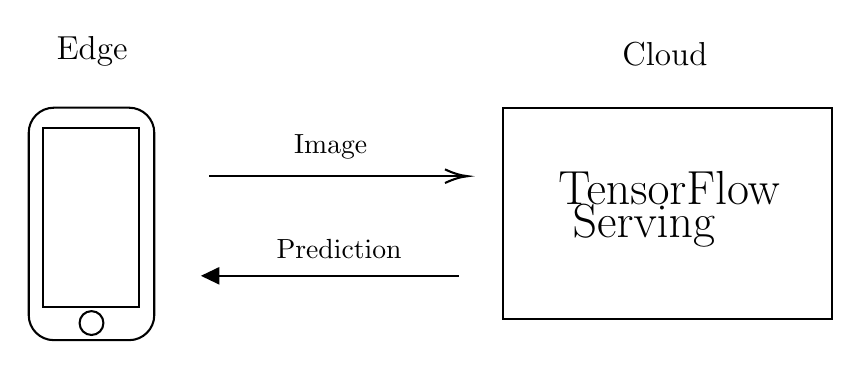
\begin{tikzpicture}[x=0.75pt,y=0.75pt,yscale=-1,xscale=1]
%uncomment if require: \path (0,300); %set diagram left start at 0, and has height of 300

\draw   (69.5,176) -- (115.5,176) -- (115.5,262) -- (69.5,262) -- cycle ;
\draw   (62.5,178.1) .. controls (62.5,171.42) and (67.92,166) .. (74.6,166) -- (110.9,166) .. controls (117.58,166) and (123,171.42) .. (123,178.1) -- (123,265.9) .. controls (123,272.58) and (117.58,278) .. (110.9,278) -- (74.6,278) .. controls (67.92,278) and (62.5,272.58) .. (62.5,265.9) -- cycle ;
\draw   (87,269.75) .. controls (87,266.57) and (89.57,264) .. (92.75,264) .. controls (95.93,264) and (98.5,266.57) .. (98.5,269.75) .. controls (98.5,272.93) and (95.93,275.5) .. (92.75,275.5) .. controls (89.57,275.5) and (87,272.93) .. (87,269.75) -- cycle ;
\draw    (149.48,199) -- (272,199) ;
\draw [shift={(274,199)}, rotate = 540] [color={rgb, 255:red, 0; green, 0; blue, 0 }  ][line width=0.75]    (10.93,-3.29) .. controls (6.95,-1.4) and (3.31,-0.3) .. (0,0) .. controls (3.31,0.3) and (6.95,1.4) .. (10.93,3.29)   ;

\draw    (147.48,247) -- (270,247) ;

\draw [shift={(145.48,247)}, rotate = 360] [fill={rgb, 255:red, 0; green, 0; blue, 0 }  ][line width=0.75]  [draw opacity=0] (8.93,-4.29) -- (0,0) -- (8.93,4.29) -- cycle    ;
\draw   (291,166) -- (449.5,166) -- (449.5,268) -- (291,268) -- cycle ;

\draw (208,185) node  [align=left] {Image};
\draw (212,234) node  [align=left] {Prediction};
\draw (93,139) node  [align=left] {{\large Edge}};
\draw (369,140) node  [align=left] {{\large Cloud}};
\draw (371,215) node  [align=left] {{\LARGE TensorFlow}\\{\LARGE  \  Serving}};


\end{tikzpicture}
\caption{placeholder}
\label{fig:cloud}
\end{figure}
\begin{figure}[H]
\centering



\tikzset{every picture/.style={line width=0.75pt}} %set default line width to 0.75pt        

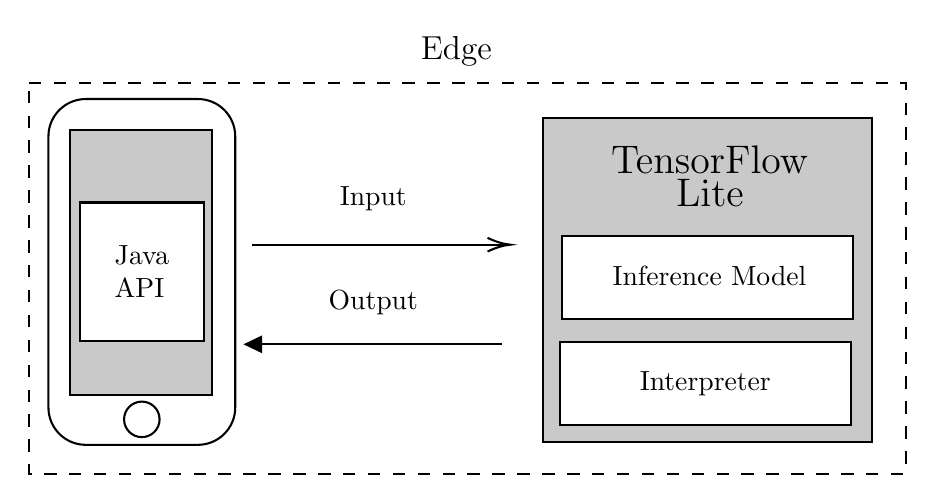
\begin{tikzpicture}[x=0.75pt,y=0.75pt,yscale=-1,xscale=1]
%uncomment if require: \path (0,300); %set diagram left start at 0, and has height of 300

%Shape: Rectangle [id:dp13292222689234756] 
\draw  [fill={rgb, 255:red, 201; green, 201; blue, 201 }  ,fill opacity=1 ] (61.91,111.69) -- (130.34,111.69) -- (130.34,239.63) -- (61.91,239.63) -- cycle ;
%Rounded Rect [id:dp7897713915001106] 
\draw   (51.5,114.82) .. controls (51.5,104.88) and (59.56,96.82) .. (69.5,96.82) -- (123.5,96.82) .. controls (133.44,96.82) and (141.5,104.88) .. (141.5,114.82) -- (141.5,245.43) .. controls (141.5,255.37) and (133.44,263.43) .. (123.5,263.43) -- (69.5,263.43) .. controls (59.56,263.43) and (51.5,255.37) .. (51.5,245.43) -- cycle ;
%Shape: Ellipse [id:dp9670901006981827] 
\draw   (87.95,251.16) .. controls (87.95,246.43) and (91.78,242.6) .. (96.5,242.6) .. controls (101.22,242.6) and (105.05,246.43) .. (105.05,251.16) .. controls (105.05,255.88) and (101.22,259.71) .. (96.5,259.71) .. controls (91.78,259.71) and (87.95,255.88) .. (87.95,251.16) -- cycle ;
%Straight Lines [id:da9993479608904674] 
\draw    (149.48,167) -- (272,167) ;
\draw [shift={(274,167)}, rotate = 540] [color={rgb, 255:red, 0; green, 0; blue, 0 }  ][line width=0.75]    (10.93,-3.29) .. controls (6.95,-1.4) and (3.31,-0.3) .. (0,0) .. controls (3.31,0.3) and (6.95,1.4) .. (10.93,3.29)   ;

%Straight Lines [id:da5401559459790608] 
\draw    (147.48,215) -- (270,215) ;

\draw [shift={(145.48,215)}, rotate = 360] [fill={rgb, 255:red, 0; green, 0; blue, 0 }  ][line width=0.75]  [draw opacity=0] (8.93,-4.29) -- (0,0) -- (8.93,4.29) -- cycle    ;
%Shape: Rectangle [id:dp45054130026891115] 
\draw  [fill={rgb, 255:red, 201; green, 201; blue, 201 }  ,fill opacity=1 ] (290,106) -- (448.5,106) -- (448.5,262) -- (290,262) -- cycle ;
%Shape: Rectangle [id:dp21016153851852382] 
\draw  [fill={rgb, 255:red, 255; green, 255; blue, 255 }  ,fill opacity=1 ] (299,163) -- (439,163) -- (439,203) -- (299,203) -- cycle ;
%Shape: Rectangle [id:dp8946256165796296] 
\draw  [fill={rgb, 255:red, 255; green, 255; blue, 255 }  ,fill opacity=1 ] (298,214) -- (438,214) -- (438,254) -- (298,254) -- cycle ;
%Shape: Rectangle [id:dp1345031923489386] 
\draw  [dash pattern={on 4.5pt off 4.5pt}] (42,89) -- (464.5,89) -- (464.5,277.4) -- (42,277.4) -- cycle ;
%Shape: Rectangle [id:dp7242946292477495] 
\draw  [fill={rgb, 255:red, 255; green, 255; blue, 255 }  ,fill opacity=1 ] (66.56,146.69) -- (126.44,146.69) -- (126.44,213.56) -- (66.56,213.56) -- cycle ;

% Text Node
\draw (208,145) node  [align=left] {Input};
% Text Node
\draw (248,74) node  [align=left] {{\large Edge}};
% Text Node
\draw (370,134) node  [align=left] {{\Large TensorFlow}\\{\Large  \ \ \ \ \ Lite}};
% Text Node
\draw (370,182) node  [align=left] {Inference Model};
% Text Node
\draw (208,195) node  [align=left] {Output};
% Text Node
\draw (368,234) node  [align=left] {Interpreter};
% Text Node
\draw (96.5,180.12) node  [align=left] {Java\\ API};


\end{tikzpicture}
\caption{placeholder}
\label{fig:edge}
\end{figure}
\subsection{Hardware}
\subsubsection{Edge}
As the edge device we will use the Oneplus 6T. This state of the art smartphones is powered by Qualcomm Snapdragon 845 CPU(Octa-core, up to 2.8 GHz), Adreno 630 GPU, 8 GB of memory and runs on OxygenOS, which is based on Android 9.
\subsubsection{Cloud}
The Nvidia DGX-1 will serve as the cloud-backend for the experiments. This server consists of 8$\times$Tesla V100 providing 1000 TFLOPS as well as 256 GB GPU memory and 512 GB system memory.
\subsection{Frameworks}
Two open-source frameworks will be used for the experiments.
\subsubsection{TensorFlow Lite}
TensorFlow Lite was developed for mobile and embedded devices and is a lightweight solution of TensorFlow.
At the moment only inference is supported and not the training of the models.
It supports acceleration with GPU or other accelerators as well was portability to Android, iOS and other IoT devices.


To use model in TensorFlow Lite models need to be converted to the \emph{tflite} format.
\subsubsection{TensorFlow Serving}
TensorFlow Serving is a framework to serve machine learning models in production envrionments. 

TensorFlow Serving supports two APIs: gRPC and REST
\subsection{Models}
We will use two different image classification model for the experiment, one optimized for mobile deployment and the other optimized for the highest accuracy.

\subsubsection{MobileNetV2}
MobileNetV2 is a successor of MobileNetV1 and is "specifically tailored for mobile and resource
constrained environments" \cite{DBLP:journals/corr/abs-1801-04381}. The authors do this by "significantly decreasing the number of operations and the memory needed while retaining the same accuracy"  \cite{DBLP:journals/corr/abs-1801-04381} and introducing a new layer module called "the
inverted residual with linear bottleneck" \cite{DBLP:journals/corr/abs-1801-04381}.

\subsubsection{Inception V4}
Inception V4 is a large image classification model with high accuracy but also with a high number of parameters leading to higher inference times than MobileNet.
%%Insert Tabelle mit overview über model specs
\begin{table}[]
\caption{Overview of used models}
\begin{tabular}{|l|l|l|l|l|}
\hline
\rowcolor[HTML]{C0C0C0} 
 & {\color[HTML]{000000}Parameters} & {\color[HTML]{000000} Top-5 Accuracy \cite{modelspecs}} & Input Size & TF Lite Model Size \\ \hline
\cellcolor[HTML]{C0C0C0}{\color[HTML]{000000} Inception V4} & wet & 95.1\% & 299 & 107.7 MB \\ \hline
\cellcolor[HTML]{C0C0C0}{\color[HTML]{000000} Mobilenet V2 1.0} & 3470000 \cite{mobilenetspecs}& 90.6\% & 224 & 14.0 MB \\ \hline
\cellcolor[HTML]{C0C0C0}\begin{tabular}[c]{@{}l@{}}Mobilenet V2 1.0\\ quantized\end{tabular} & 3470000 \cite{mobilenetspecs}& 89.9\% & 224 & 3.4 MB \\ \hline
\end{tabular}
\end{table}


For the experiments we both evaluate the normal float version as well as the quantized version using int8.
\subsection{Android Benchmark Application}
In order to perform the inference process on the edge devices we developed a benchmark android application using Kotlin. 

\begin{figure}[H]
\centering
\includegraphics[width=0.9\textwidth]{./Bilder/FlowChart_App.png}
\caption{Flowchart of the benchmark Application}
\label{fig:app}
\end{figure}
In figure \ref{fig:app} the workflow to get perform the inference is seen. First, a image needs to be selected, either an existing one from the gallery or a new one shot with the camera of the phone. Afterwards the image classification model needs to be chosen. Now the user selects whether the inference should be performed on the cloud-backend or directly on the edge device, in this case a android phone. Afterwards the selected image needs to be preprocessed according to the selected model, inference mode (edge/cloud) and for the case of cloud inference, if the image should be preprocessed on the cloud or on the edge. Finally the inference is performed resulting and after finishing the labels with the highest probabilities are presented to the user as the prediction for the given image. The image preprocessing step and the inference step are seperated to allow better measurements of these steps.
\subsubsection{Edge Inference}

\subsubsection{Cloud Inference}
\section{Instantiation}
We run parameter configuration 100 times to reduce 
We change the configurations of the following parameters:
\paragraph{Image Size}
Image Size: We evaluate the performance of the small(YxY), medium(YxY) and large(YxY) images. This way the effect of image size on the performance of the preprocessing step can assessed.
\paragraph{Batch Size}
We experiment with the following batch sizes: 1, 2, 4 , 8, 16, 32, 64.
\paragraph{NNAPI}
The Android Neural Network API (NNAPI)
is "designed for running computationally intensive operations for machine learning on mobile devices" \cite{NNAPI} and can be used by TensorFlow Lite to improve inference performance. Therefore we take a look into the effect of this framework.
\paragraph{GPU Usage}
Since the latest release of TensorFlow Lite(version xxx) GPU usage on Android is supported. 

\subsection{Measurements}
We conduct the measurement either directly in the source code or by using Android Studio Profiler.
\subsubsection{Inference Time}
To measure inference time we need to  distinguish between edge and cloud inference. To measure edge inference we measure the time the TensorFlow Lite interpreter needs to run the inference operation on the loaded model given the input image.
To measure the cloud inference time we need to measure two latencies. The first latency is the server latency. This server latency describes the time difference between the point where TensorFlow Serving receives the inference request and the point in time where TensorFlow Serving send the response back to the client.



The second latency is called the total latency and describes the time difference between the moment the client sent the request to TensorFlow Serving and the moment it received its response, including the network latency.
These two latencies are illustrated in figure \ref{fig:serverLat}.
The total latency is be measured by simply measure the time needed to call the \emph{predict} function of TensorFlow Serving.
Since TensorFlow Serving does not output the server latency, we needed to tweak the source code of gRPC, which is the underlying protocol of TensorFlow Serving. gRPC already logs this latency, so we adjust the source code to out this latency when a call to TensorFlow Serving is finished, repackage the source code and change to dependencies of TensorFlow Serving accordingly.
\begin{figure}[H]
\centering
\includegraphics[width=0.7\textwidth]{./Bilder/server_latency.png}
\caption{Measurement of server and total latency for cloud inference}
\label{fig:serverLat}
\end{figure}
\subsubsection{Energy Consumption}
Since Android Studio Profiler only estimates the energy consumption in the form of low, medium and high, the tool is not fit to provide empiric measurements. The Trepn Power Profiler would provide such measurements, but does not support the device used for the experiments (Oneplus 6T).
\subsubsection{CPU Usage}

\subsubsection{Memory Usage}
The Memory Profiler is part of Android Studio Profiler and shows the memory consumption of the app it is profiling. Memory allocations by the operating system or other apps are not recorded. Besides recording the total amount of memory allocated the profiler also tracks the different categories, for example memory allocated by Java/Kotlin code.
\subsubsection{GPU Usage}
If a GPU or a another accelator is available their usage is of interest.
\subsubsection{Throughput}
In order to measure throughput we 
\subsubsection{Data Consumption}
Android Studio Profiler provides a tool named Network Profiler, which displays all the data sent and recieved.
\section{Results and Evaluation}
\begin{itemize}
    \item Haufen Graphen
    \item Was kann man aus Graphen schließen?
    \item Handlungsempfehlung
\end{itemize}
\endinput 
